\documentclass[11pt]{article}
\usepackage[utf8]{inputenc}
%\usepackage[latin1]{inputenc}
\usepackage[spanish,es-tabla]{babel}
\usepackage{anysize}
\usepackage{graphicx} 
\usepackage{amsmath}
\usepackage{float}
\usepackage{tikz}
\usepackage{color}
\usepackage{multicol}
\usepackage{multirow}
\usepackage{array}
\usepackage{siunitx}
\usepackage[autostyle,spanish=mexican]{csquotes}
\usepackage{xcolor}
\usepackage{caption}
\captionsetup{font=scriptsize,labelfont=scriptsize}
\usepackage{listings}
\lstset{
basicstyle=\ttfamily,
columns=flexible,
breaklines=true
}

\definecolor{ao}{rgb}{0.0, 0.5, 0.0}
\definecolor{bisque}{rgb}{1.0, 0.89, 0.77}
\definecolor{amber}{rgb}{1.0, 0.75, 0.0}
\definecolor{armygreen}{rgb}{0.29, 0.33, 0.13}
\definecolor{alizarin}{rgb}{0.82, 0.1, 0.26}
\definecolor{cadetblue}{rgb}{0.37, 0.62, 0.63}
\definecolor{deepblue}{rgb}{0,0,0.5}
\definecolor{brown}{rgb}{0.59, 0.29, 0.0}
\definecolor{OliveGreen}{rgb}{0,0.25,0}

\definecolor{Code}{rgb}{0,0,0}
\definecolor{Keywords}{rgb}{255,0,0}
\definecolor{Strings}{rgb}{255,0,255}
\definecolor{Comments}{rgb}{0,0,255}
\definecolor{Numbers}{rgb}{255,128,0}

\DeclareCaptionFormat{listing}{\colorbox{gray}{\parbox{0.99\textwidth}{#1#2#3}}}
%\captionsetup[lstlisting]{format=listing,labelfont=white,textfont=white}
\renewcommand{\lstlistingname}{Código}

\lstdefinestyle{codigopython}{%
  language=Python,                % choose the language of the code
  %basicstyle=\footnotesize\small,       % the size of the fonts that are used for the code
  numbers=left,                   % where to put the line-numbers
  numberstyle=\scriptsize,      % the size of the fonts that are used for the line-numbers
  stepnumber=1,                   % the step between two line-numbers. If it is 1 each line will be numbered
  numbersep=5pt,                  % how far the line-numbers are from the code
  backgroundcolor=\color{white},  % choose the background color. You must add \usepackage{color}
  showspaces=false,               % show spaces adding particular underscores
  showstringspaces=false,         % underline spaces within strings
  showtabs=false,                 % show tabs within strings adding particular underscores
  frame=single,   		% adds a frame around the code
  tabsize=2,  		% sets default tabsize to 2 spaces
  captionpos=t,   		% sets the caption-position to bottom
  breaklines=true,    	% sets automatic line breaking
  breakatwhitespace=false,    % sets if automatic breaks should only happen at whitespace
  escapeinside={\#},  % if you want to add a comment within your code
  stringstyle =\color{OliveGreen},
  texcl = true,
  %otherkeywords={{as}},             % Add keywords here
  keywordstyle = \color{blue},
  commentstyle = \color{black},
  identifierstyle = \color{black},
  % literate=%
  %         {á}{{\'a}}1
  %         {é}{{\'e}}1
  %         {í}{{\'i}}1
  %         {ó}{{\'o}}1
  %         {ú}{{\'u}}1
  %
  %keywordstyle=\ttb\color{deepblue}
  %fancyvrb = true,
literate={0}{{\textcolor{red}{0}}}{1}%
            {1}{{\textcolor{red}{1}}}{1}%
            {2}{{\textcolor{red}{2}}}{1}%
            {3}{{\textcolor{red}{3}}}{1}%
            {4}{{\textcolor{red}{4}}}{1}%
            {5}{{\textcolor{red}{5}}}{1}%
            {6}{{\textcolor{red}{6}}}{1}%
            {7}{{\textcolor{red}{7}}}{1}%
            {8}{{\textcolor{red}{8}}}{1}%
            {9}{{\textcolor{red}{9}}}{1}%
            {.0}{{\textcolor{red}{.0}}}{2}% Following is to ensure that only periods
            {.1}{{\textcolor{red}{.1}}}{2}% followed by a digit are changed.
            {.2}{{\textcolor{red}{.2}}}{2}%
            {.3}{{\textcolor{red}{.3}}}{2}%
            {.4}{{\textcolor{red}{.4}}}{2}%
            {.5}{{\textcolor{red}{.5}}}{2}%
            {.6}{{\textcolor{red}{.6}}}{2}%
            {.7}{{\textcolor{red}{.7}}}{2}%
            {.8}{{\textcolor{red}{.8}}}{2}%
            {.9}{{\textcolor{red}{.9}}}{2}%
            {\ }{{ }}{1}% handle the space
        ,%
        %mathescape=true
        %escapeinside={*@}
        escapeinside={A_}{_B}
}
\renewcommand*{\theenumi}{\thesection.\arabic{enumi}}
\renewcommand*{\theenumii}{\theenumi.\arabic{enumii}}
\marginsize{1cm}{2cm}{0cm}{2cm}  
\newcommand{\letraconsola}[1]{\texttt{#1}}
\title{Uso de paquetes para formateo de datos \\ Curso de Física Computacional}
\author{M. en C. Gustavo Contreras Mayén}
\date{ }
\begin{document}
\maketitle
\fontsize{14}{20}\selectfont
\section{Introducción.}
Cuando se inicia la programación con \letraconsola{python} suele suceder que en un primer momento nos enfoquemos a los resultados que nos devuelve el algoritmo que estemos usando, más cuando los resultados se presentan en la terminal a modo de tabla.
\par
Por ejemplo: en el ejercicio donde calculamos la aproximación de la función $\sin(x)$ mediante una suma finita, los resultados que presentamos en la terminal son parecidos a la siguiente tabla:
\begin{figure}[H]
    \centering
    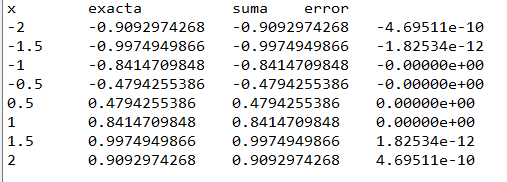
\includegraphics{Imagenes/instalacion_paquete_python_03.png}
    \caption{Detalle de la tabla sin formato en la terminal}
    \label{fig:figura_01}
\end{figure}
Como podemos revisar de la tabla anterior, se cumple con la presentación de datos en la terminal, pero existe una dificultad visual para leer correctamente los encabezados, a pesar de que se incluyó en el código, un tabulador que separase los mismos.
\par
Una de la grandes ventajas de \letraconsola{python} es que contamos con una enorme cantidad de paquetes que se han desarrollado para mejorar los programas, uno de esos paquetes que tiene que ver con una salida de datos formateada, es el paquete \letraconsola{Pretty Table}, que normalmente no está instalada de manera predeterminada, por lo que veremos cómo se instala en nuestro equipo.
\par
Como utilizamos \letraconsola{Anaconda} como el IDE para \letraconsola{python}, la mejor manera de instalar un paquete es por medio de la consola y ejecutar la sentencia respectiva, por lo que abrimos una ventana de comandos (terminal) de \letraconsola{Anaconda}:
\subsection{En Windows.}
\begin{enumerate}
\item En el menú de inicio, localizamos el correspondiente ícono para la terminal de \letraconsola{Anaconda}:
\begin{figure}[H]
    \centering
    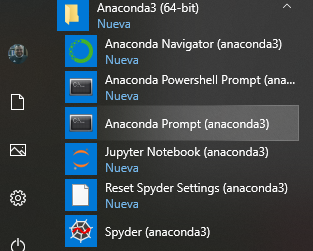
\includegraphics[scale=0.6]{Imagenes/instalacion_paquete_python_01.png}
    \caption{En el Menú Inicio está el acceso a la terminal de Anaconda.}
    \label{fig:figura_02}
\end{figure}
\item Es importante señalar que cuando usamos \letraconsola{Anaconda}, la terminal se abrirá en el entorno virtual \letraconsola{base}, es decir, la instalación del paquete se realiza dentro de este entorno, no quedará instalado de manera global.
\par
Si queremos usar el paquete de manera global, tendremos que seguir este procedimiento desde una terminal de nuestro sistema, para usar \letraconsola{pip}:
\\
\verb|pip install PrettyTable|
\item El comando que debemos de escribir en la consola para que se descargue e instale el paquete \letraconsola{Pretty Table} es el siguiente:
\\
\verb|conda install -c conda-forge prettytable|
\\
En la terminal quedaría así:
\begin{figure}[H]
    \centering
    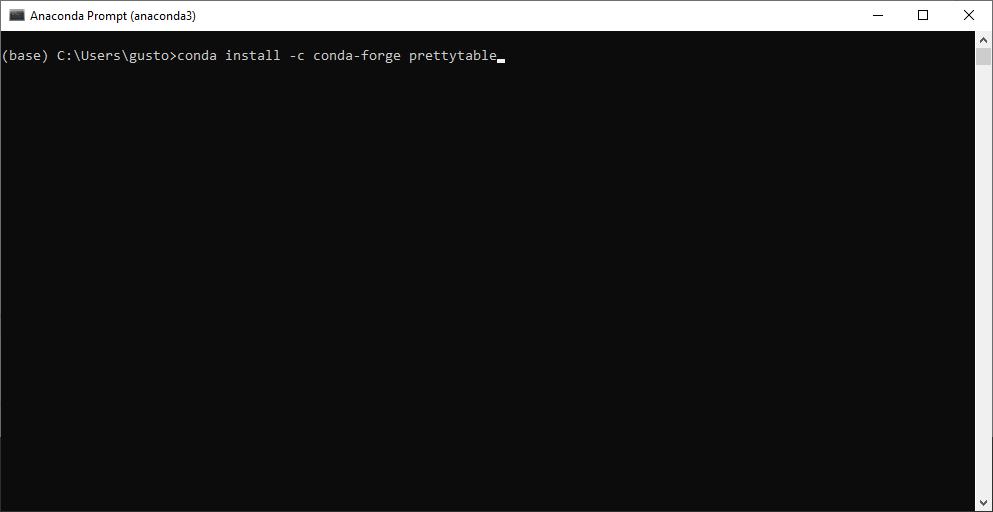
\includegraphics[scale=0.6]{Imagenes/instalacion_paquete_python_02.png}
    \caption{Escribimos el comando y al presionar Enter, veremos que se realiza la descarga e instalación del paquete.}
    \label{fig:figura_03}
\end{figure}
\end{enumerate}
\section{En Linux/iOS.}
Para instalar el paquete en sistemas Linux o iOS, el procedimiento es similar:
\begin{enumerate}
\item Abrimos una terminal y llamamos al entorno virtual \letraconsola{base} que es en donde está instalado \letraconsola{Anaconda}, escribimos el siguiente comando:
\\
\medskip
\verb|conda activate base|
\\
\medskip
Nos daremos cuenta de que el entorno ya está cargado por que aparece como prefijo el nombre del entorno entre paréntesis en el prompt de la terminal de comandos. En caso de que tengas una configuración diferente y no recuperes el entorno virtual, revisa la documentación de \letraconsola{Anaconda}.
\begin{figure}[H]
    \centering
    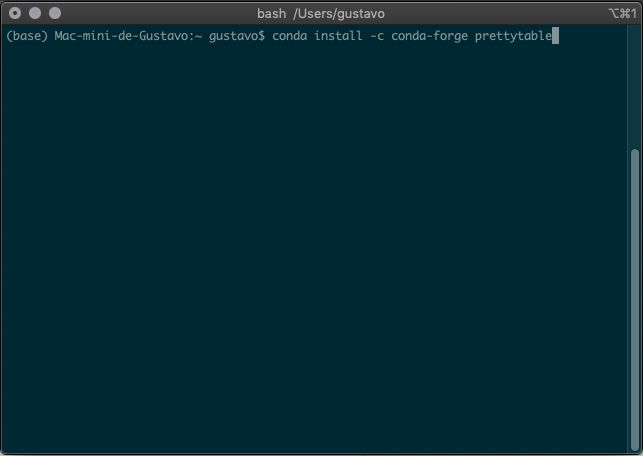
\includegraphics[scale=0.5]{Imagenes/instalacion_paquete_python_05.png}
    \caption{Terminal con el entorno virtual \letraconsola{base}.}
    \label{fig:figura_05}
\end{figure}
\item Escribimos el mismo comando \verb|conda install -c conda-forge prettytable| y presionamos Enter.
\begin{figure}[H]
    \centering
    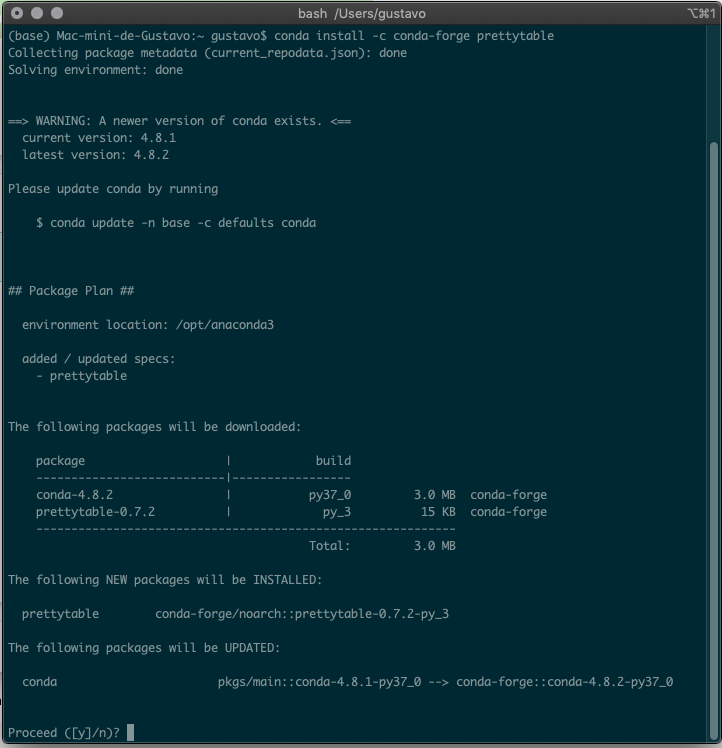
\includegraphics[scale=0.5]{Imagenes/instalacion_paquete_python_06.png}
    \caption{Comando para descargar e instalar \letraconsola{Pretty Table}.}
    \label{fig:figura_06}
\end{figure}
\item Debemos de confirmar la operación y con ello se verá el avance para la descarga e instalación:
\begin{figure}[H]
    \centering
    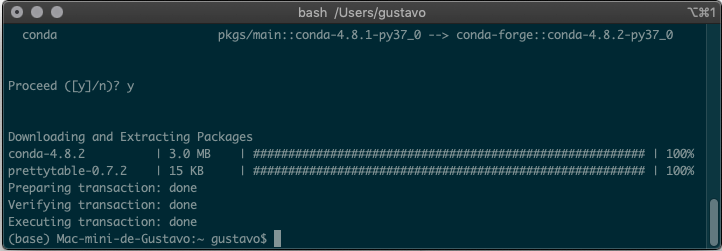
\includegraphics[scale=0.5]{Imagenes/instalacion_paquete_python_07.png}
    \caption{Resumen de la instalación del paquete.}
    \label{fig:figura_07}
\end{figure}
\end{enumerate}
\newpage
\section{Uso del paquete en el código.}
\begin{enumerate}
\item Una vez instalado el paquete, ya podemos utilizarlo dentro de nuestro código en \letraconsola{python}:
\begin{lstlisting}[style=codigopython]
from prettytable import PrettyTable
import math

def error_relativo(exacto, aproximado):
    return math.fabs(math.sin(exacto)- aproximado)/math.sin(exacto)*100

x = [-2, -1.5, -1, -0.5, 0.5, 1, 1.5, 2]
n = 10

t = PrettyTable(['x', 'exacta', 'suma' , 'error'])

for j in x:
    suma = j
    term = j
    for i in range(2, n):
        term = (-term *j*j)/((2*i-1)*(2*i-2))
        suma = suma + term
    t.add_row([j, math.sin(j), suma, error_relativo(j, suma)])

print(t)
\end{lstlisting}
\item Revisemos cómo se usa el paquete \letraconsola{Pretty Table}:
\begin{enumerate}
\item En la línea $1$ del código se carga el paquete \letraconsola{prettytable}, se ocupa la función \letraconsola{Pretty Table}.
\item En la línea $10$ se crea el objeto \letraconsola{Pretty Table} en una variable $t$, se incluyen los encabezados que tendrá nuestra tabla.
\item En la línea $18$ se van incluyendo los renglones de la tabla, mediante la función \letraconsola{add\_row}, en nuestro caso, agregamos los valores que se obtienen del código que nos aproxima el valor de la función.
\item En la línea $20$ se presenta el objeto \letraconsola{Pretty Table} en la terminal, mediante la función \verb|print(t)|.
\end{enumerate}
\end{enumerate}
\section{Salida en la terminal}
\begin{enumerate}
\item En Windows: La tabla que se muestra ya con un mejor formato es la siguiente:
\begin{figure}[H]
    \centering
    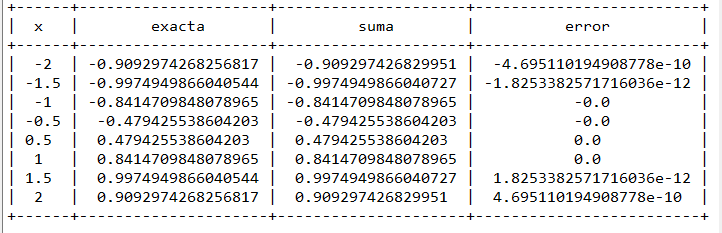
\includegraphics[scale=0.8]{Imagenes/instalacion_paquete_python_04.png}
    \caption{Detalle de la tabla ya con un formato más amigable.}
    \label{fig:figura_04}
\end{figure}
\item En Linux/iOS: La tabla es la siguiente:
\begin{figure}[H]
    \centering
    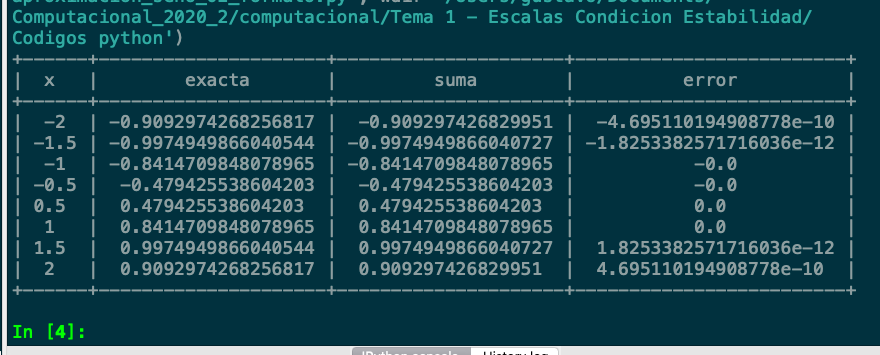
\includegraphics[scale=0.4]{Imagenes/instalacion_paquete_python_08.png}
    \caption{La misma tabla con formato en Linux/iOS.}
    \label{fig:figura_08}
\end{figure}
\end{enumerate}
Considera que es posible \enquote{elaborar} manualmente un formato como el que se muestra en la figura anterior, es decir, podemos hacer la decoración de salida para que se muestre, pero ello implica que tengamos que dedicarle un buen rato para ajustar cada elemento con alguna instrucción de \letraconsola{python}.
\par
Si revisamos en la documentación oficial, podremos encontrar una variedad de paquetes que nos van a reducir el trabajo y con ello, mejorar mucho nuestras técnicas de programación, así como un mayor dominio del lenguaje \letraconsola{python.}
\end{document}